\chapter{Materiál a metody}

\section{Vymezení problému}

\fixme{Vlastními slovy}

Jako vzorový příklad si můžeme vzít tento zrcadlový světlovod - plášť komolého jehlanu s odříznutou špičkou a podstavou; v limitním případě může jít o hranol. Ze strany odříznuté špičky svítí plošný zdroj světla. Paprsky se šíří ve směru k odříznuté podstavě, a to jak přímo, tak i odrazy od stěn. Naším cílem je pochopit nejenom celkovou funkci této optické soustavy, ale i detaily o vystupujícím světle.

Tato práce je pouze pokusem demonstrujícím jistou myšlenku. Proto je vhodné nejprve problém co nejvíce zjednodušit, a až pokud se naše hypotéza ověří, uvažovat o zobecnění.

Omezíme se tedy nejprve na 2D řez, respektive na 2D optický systém. Náš příklad se tudíž zjednoduší na zdroj světla v podobě úsečky a světlovod ve formě lichoběžníku (limitně obdélníku) s odříznutými čely, tj. de facto dvěma úsečkami představujícími zrcadla.

\begin{center}
    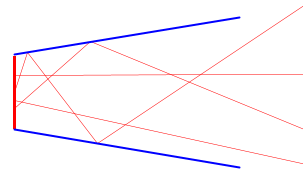
\includegraphics[scale=0.7]{2.1_priklad.png}\\
    \todo{Popisek obrázku; formát popisku}\\
\end{center}

Naopak nebudeme zavádět zjednodušení typické u zobrazovací optiky - náhradu plošného (lineárního) zdroje světla bodovým. Nezobrazovací optika je typická právě prací se světelnými zdroji, jejichž velikost je nezanedbatelná vzhledem k velikosti optického systému.

Dále budeme pracovat čistě s paprskovou představou světla, tj. nebudeme uvažovat jeho vlnové vlastnosti. To je adekvátní u makroskopických optických soustav (např. světlomety), naopak neadekvátní např. při studiu optických vláken. Takové typy nezobrazovací optiky tedy z analýzy vědomě
vypouštíme.

Budeme uvažovat pouze dokonalý zrcadlový odraz nebo dokonalou absorpci světla. V praxi by bylo třeba též zahrnout lom světla, rozptyl (odraz od matného povrchu), částečný odraz, případně další jevy. Nebudeme uvažovat závislost optické interakce na barvě (vlnové délce) světla nebo jeho polarizaci. Budeme předpokládat, že každý paprsek nese stejný elementární optický výkon. Optický výkon (světelný tok) celého světelného zdroje je pak dán prostým součtem elementárních optických výkonů.

\pic{Odraz na lineárním zrcadlu, absorbce, další}


Sledovaná optická soustava může být velmi jednoduchá jako v uvedeném případě, ale může také obsahovat neomezené množství lineárních zrcadel (k aproximaci křivých povrchů), lineárních světelných zdrojů a
lineárních absorbérů (clon). Důležité je, že předem není známo, jak bude paprsek optickou soustavou postupovat. To je zásadní rozdíl oproti zobrazovací optice, např. teleskopu se dvěma čočkami, kde je předem zřejmé, že paprsek světla se nejdřív lomí na přední ploše první čočky, pak na zadní ploše první čočky, pak na přední ploše druhé čočky a nakonec na zadní ploše druhé čočky. Tato apriorní znalost podstatně zjednodušuje analýzu zobrazovací optiky -- a neznalost komplikuje analýzu nezobrazovací optiky.



\section{Analýza systému}

Budeme používat dvourozměrný kartézský souřadný systém (systém $Oxy$), 
přičemž počátek soustavy $O$ můžeme umístit kamkoliv. Předpokládáme, že světlo
se primárně šíří ve směru $+x$, světelný paprsek tak můžeme
popsat rovnicí: 

$$y = kx + q$$

K analýze paprsků v místech, kde protínají osu $y$ systému $Oxy$,
slouží \emph{prostorovo-fázový diagram}. 


\todo{Vysvětlení a obrázky: jeden paprsek,
vějíř paprsků vycházejících z jednoho bodu, svazek rovnoběžných paprsků,
plošný zdroj světla. Vysvětlení může být na diagramu úhel-místo,
případně směrnice-místo; uvést, že nejpraktičtější je diagram "sinus
úhlu"-místo, resp. "y složka směrového vektoru paprsku"-místo.}

\todo{Možno vysvětlit, že v případě 3D geometrie je prostorovo-fázový diagram
čtyřrozměrný (dvě prostorové, dvě úhlové veličiny), což významně
komplikuje vizualizaci. I proto omezení na 2D; pokud bude 2D analýza
neužitečná, tím spíš bude neužitečná analýza 3D.}

\todo{Ukázat, co se děje, pokud počátek systému $Oxy$ posuneme
doprava nebo doleva -- vodorovné nebo svislé "zkosení" obrazce v
prostorovo-fázovém diagramu. Pozn.: opravdové zkosení je to v případě
diagramu směrnice-místo; v případě "sinus úhlu"-místo se do zkosení
přidává i nelineární zkřivení.}

Ukázat, co se děje při odrazu na zrcadle, a to jak v případě, že je
odražen kompletní svazek, tak v případě, že je zrcadlo malé a je
odražena pouze část svazku.

Dokud platí, že při interakci s optickým povrchem jeden vstupní paprsek
vytváří jeden výstupní paprsek, je plocha obrazce tvořeného všemi
paprsky v prostorovo-fázovém diagramu konstantní nezávisle na volbě
počátku systému $Oxy$. To je zákon zachování étendue; étendue
je plocha obrazce v prostorovo-fázovém diagramu.

Zjednodušeně lze říct, že součin prostorového a úhlového rozsahu je
konstantní. Přesněji řečeno to platí jen pro svazek paprsků
diferenciální velikosti (nekonečně malý rozsah v úhlové i prostorové
souřadnici), ale jelikož celé étendue je složeno z nekonečně mnoha
svazků diferenciální velikosti, platí to integrálně (v sumě) i pro celý
svazek paprsků.

\pic{Možno dovysvětlit obrázkem -- těsně u světelného zdroje
je prostorový rozsah světelného svazku malý a úhlový velký; daleko od
světelného zdroje se světlo hodně roztáhne, tj. prostorový rozsah je
velký, ale lokálně je úhlový rozsah malý.}

Z toho se dá například pro náš jednoduchý světlovod odhadnout, že čím
bude výstupní otvor větší, tím bude mít vystupující světlo menší úhlový
rozsah -- tady by bylo dobré dát obrázky.

Pokud ale chceme za jednoduchý světlovod umístit další optický člen, je
užitečné znát nejenom globální chování veškerého světla vycházejícího ze
světlovodu, ale i lokální detaily chování -- například jaké světlo
vystupuje ze středu výstupního otvoru, poblíž okrajů apod. To by měl
zodpovědět prostorovo-fázový diagram.

Kromě vizuálního hodnocení prostorovo-fázového diagramu je při analýze
optického systému vhodné znát i další údaje, a to:
-- étendue
-- celkový světelný tok procházející osou y v systému Oxy
-- rozložení svítivosti, tj. kolik světelného toku jde do kterého směru

Poznámka k jednotkám:
- Optický výkon, přesněji zářivý výkon, se udává ve wattech [$W$]. V
případě světelnětechnických výpočtů, kde se bere v potaz i citlivost
lidského oka na světlo různých vlnových délek, se přechází z wattů [$W$]
na lumeny [$lm$]. V případě aproximace světla konečným množstvím paprsků
můžeme říkat, že paprsek nese elementární optický výkon ve wattech resp.
lumenech.
- Jelikož je étendue součinem prostorového a úhlového rozsahu, často se
za jednotku étendue bere metr čtverečný krát steradián [$m^2 \cdot sr$]. Při
přechodu na 2-D optický systém bude jednotkou metr krát radián [$m \cdot rad$].
Pozorný čtenář by mohl namítnout, že prostorovo-fázový diagram,
kde se étendue počítá, má osu "sinus úhlu" a nikoliv "úhel". To na věci
nic nemění, jen je třeba pečlivě formulovat, jak se má jednotka "radián"
v jednotce étendue chápat.
- Svítivost je úhlová hustota světla uváděná v lumenech na steradián
[$lm/sr$] čili kandelách [$cd$]; v případě radiometrických veličin hovoříme
o zářivosti s jednotkou watt na steradián [$W/sr$]. Po přechodu na 2-D
optický systém bude jednotkou watt na radián [$W/rad$], resp. lumen na
radián [$lm/rad$].

Také je vhodné si uvědomit, že některé poučky formulované pro 3-D
geometrii neplatí ve 2-D. Například ve 3-D platí, že osvětlenost
[$lm/m^2$] klesá se čtvercem vzdálenosti od světelného zdroje. V případě
2-D optických systémů klesá lineárně se vzdáleností od světelného
zdroje. Výsledky analýzy 2-D systémů tedy nejdou bezprostředně použít
pro 3-D systémy.



\section{Implementační prostředky}

\fixme{Vlastními slovy}

Tady bych se moc nerozepisoval. Java + Swing proto, že Javu znáte a na
Swing existuje dobrá dokumentace a je ve standardním SDK. Ad IDE - není
důležité, můžete zmínit; jediný důvod pro výběr asi je, že jej znáte.
Cílem bylo rychle prověřit použitelnost nápadu, nikoliv vytvořit
produkční software.



\section{Architektura aplikace}

\fixme{Vlastními slovy}

Popis by měl být přizpůsobený Vaší implementaci; níže je, jak bych to
implementoval já. Pokud to uznáte za vhodné, můžete jít až na
matematické vztahy, kterými něco počítáte, ale odkaz na literaturu je
dostatečný -- jde o standardní operace, které není nutné rozpitvávat.
Uznáte-li za vhodné přidat obrázky, přidejte.

Sledování paprsku (ray tracing) - ze zdroje světla se vyšle paprsek,
spočítá se průsečík se všemi objekty, vybere se nejbližší, vypočítá se
interakce (odraz, absorpce) a případně se ve sledování paprsku pokračuje
dál, dokud se nedosáhne limitního počtu interakcí (např. 1000), nebo
paprsek neopustí scénu (průsečík neexistuje).

Vizualizace chodu paprsků simulovaným systémem - tady asi jen napsat, že
k pochopení chování optického systému je užitečné vidět nejenom
abstraktní prostorovo-fázový diagram, ale i jednotlivé optické členy a
chod paprsků mezi nimi. A důležitá drobnost: pro výpočet
prostorovo-fázového diagramu potřebujete třeba statisíce paprsků, ale
pro vizualizaci chodu paprsků je vhodné nakreslit jich *maximálně* pár
set, jinak je z toho nepřehledná změť čar. Máte-li ve vizualizaci nějaký
implementačně zajímavý detail, klidně jej samozřejmě uveďte.

Výpočet prostorovo-fázového diagramu - výpočet průsečíku každého z
paprsků (jak polopřímek, tak úseček) s osou y zvoleného souřadného
systému Oxy; pokud existuje, zaznamenat průsečík + směr paprsku do
pomocného pole. Následně určit rozsah prostorovo-fázového diagramu,
rozdělit na pixely, do každého určit, kolik paprsků obsahuje.
Alternativně: rozsah prostorovo-fázového diagramu určit předem
(uživatelsky), aby byl během vizualizace rozsah pořád stejný.

Étendue: počet neprázdných pixelů. Tok: celkový počet paprsků v pomocném
poli průsečíků. Rozložení svítivosti: součet počtu paprsků v každém
diskrétním úhlu (šířky 1 pixel) prostorovo-fázového diagramu. Někde
hlásit, kolik paprsků z pomocného pole průsečíků není v
prostorovo-fázovém diagramu obsaženo.

Nevím, jestli něco obecného psát k obecné architektuře programu - to
musíte posoudit sám, jestli je tam něco mimořádně zajímavého.



% \section{Testování aplikace}
%
% \fixme{Vlastními slovy}
%
% Tato kapitolka jen pokud na ni zbyde dost času. Mohli bychom něco
% odsimulovat třeba v TracePro. Také by šlo vymodelovat jednoduché
% případy, na kterých bude zřejmé, že výsledek je správně.



\section{Ovládání aplikace}

\todo{Hlavně napsat, jak se definuje scéna. Pak případně popsat GUI.}




